% =================================================================
\section{Resultados de las pruebas}
% =================================================================
Las pruebas de carga se lanzaron con Locust desde Cartagena. Cada visita a la tienda hace
trabajar la CPU unos 40 milisegundos, para simular una página real. Los resultados completos
(CSV e informes HTML) están en la carpeta \texttt{evidencias/}.

\subsection{P1.1 ¿Cuánto aguanta un solo servidor?}
Dejamos el sistema con un único servidor y fuimos aumentando los usuarios poco a poco, de 5 en 5
y luego de 10 en 10, hasta 240.

\begin{figure}[H]
\centering
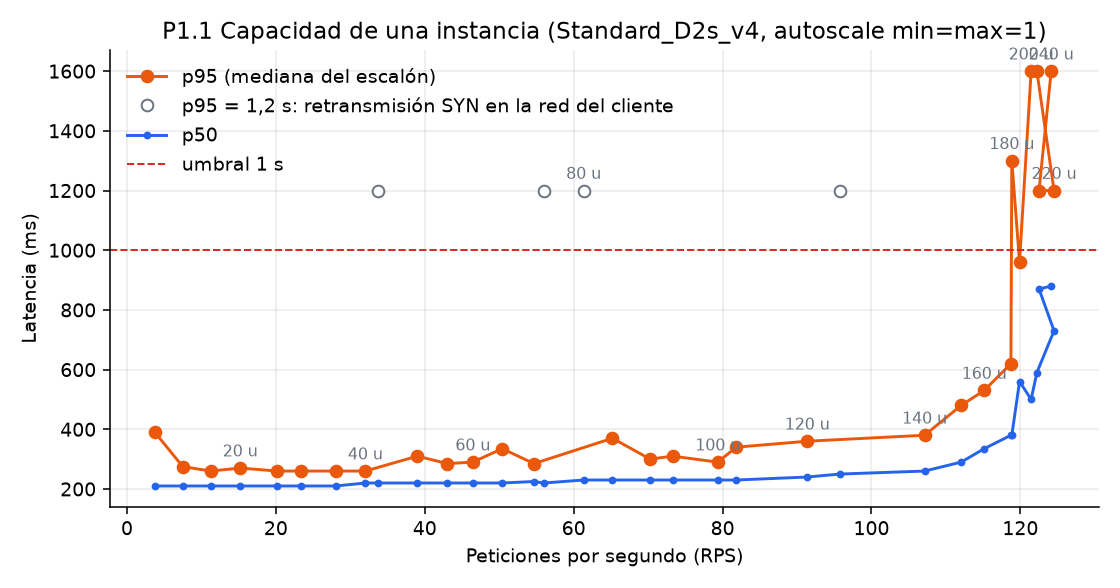
\includegraphics[width=0.82\textwidth]{figuras/p1_capacidad.png}
\caption{Tiempo de respuesta frente a peticiones por segundo con un solo servidor.}
\label{fig:cap}
\end{figure}

\begin{itemize}
  \item Un servidor atiende como máximo \textbf{unas 120 peticiones por segundo}; a partir de ahí
        la CPU llega al 98\,\% y solo crecen las esperas.
  \item \textbf{Capacidad útil: 119 peticiones/s} manteniendo el 95\,\% de las respuestas por debajo
        de 1 segundo, y \textbf{112 peticiones/s} si se exige menos de medio segundo.
  \item Al 70\,\% de CPU, el punto en que el autoscale agrega servidores, uno solo atiende unas
        60 peticiones por segundo.
  \item Los puntos grises de 1,2\,s no indican saturación: son reintentos de conexión de nuestra
        propia red doméstica. Ningún error vino del servidor.
\end{itemize}

\subsection{P1.2 ¿Escala solo cuando sube la demanda?}
Durante 35 minutos subimos la carga por escalones (de 40 a 280 usuarios) y luego la bajamos a 20,
con el autoscale configurado entre 2 y 4 servidores. En total hubo \textbf{207\,435 peticiones y
solo 0,55\,\% de errores}.

\begin{figure}[H]
\centering
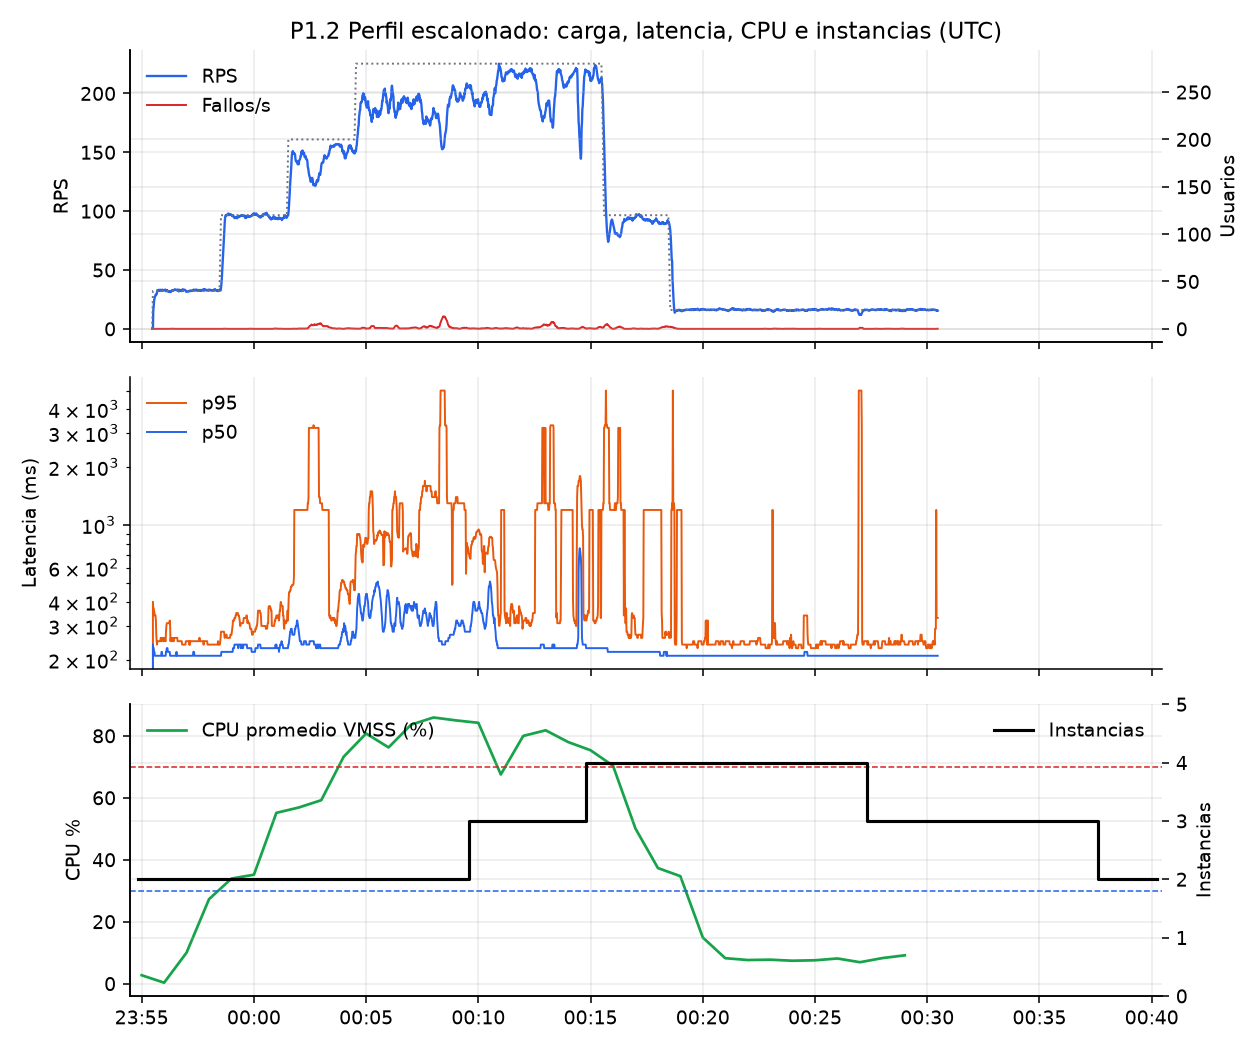
\includegraphics[width=0.86\textwidth]{figuras/p1_escalonado.png}
\caption{Carga, tiempo de respuesta, CPU y número de servidores durante la prueba (hora UTC).}
\label{fig:stair}
\end{figure}

\begin{table}[H]
\centering\small\tablaestilo
\caption{Lo que hizo el autoscale durante la prueba.}
\label{tab:autoscale}
\begin{tabular}{|c|c|p{6.4cm}|c|}
\hline
\encab \hd{Hora (UTC)} & \hd{Servidores} & \hd{Motivo} & \hd{Tardó} \\ \hline
00:09 & 2 $\rightarrow$ 3 & La CPU pasó del 70\,\% a las 00:04 & 5 min 19 s \\ \hline
00:14 & 3 $\rightarrow$ 4 & La CPU seguía alta tras la espera de 5 min & 5 min \\ \hline
00:26 & 4 $\rightarrow$ 3 & La CPU bajó del 30\,\% a las 00:20 & 6 min 49 s \\ \hline
00:37 & 3 $\rightarrow$ 2 & La CPU seguía baja tras la espera de 10 min & 10 min \\ \hline
\end{tabular}
\end{table}

\textbf{Análisis.} El autoscale funcionó como se diseñó: subió y bajó en orden, sin oscilar.
Entre las 00:16 y las 00:20 la CPU estuvo entre 30 y 70\,\% y, como esperábamos, no hizo nada.
El punto débil es el tiempo de reacción: con 280 usuarios y solo 2 servidores las respuestas se
hicieron más lentas durante unos 5 minutos, hasta que llegó el tercero. El cuarto servidor estuvo
listo justo cuando la carga empezaba a bajar. Para picos cortos, el autoscale reactivo llega tarde
(lo retomamos en la pregunta 2).

\subsection{P2 ¿Sigue funcionando si falla un servidor?}
Con una carga moderada (40 usuarios), un monitor propio hizo 10 peticiones por segundo y anotó qué
servidor respondía cada una. Así medimos exactamente cuándo deja de recibir tráfico el servidor
que falla y cuántas peticiones se pierden.

\begin{table}[H]
\centering\small\tablaestilo
\caption{Resultados de las dos pruebas de falla.}
\label{tab:p2}
\begin{tabularx}{\textwidth}{|>{\raggedright\arraybackslash\bfseries}p{4.1cm}|Y|Y|}
\hline
\encab \hd{Aspecto} & \hd{P2.1 Falla lógica} & \hd{P2.2 Falla abrupta} \\ \hline
Qué hicimos & Un servidor empieza a reportarse como enfermo & Borramos un servidor con usuarios activos \\ \hline
Deja de recibir tráfico & \textbf{a los 8 segundos} & a los 3 segundos (se apaga) \\ \hline
Errores durante la falla & \textbf{1,7\,\%}, igual que antes de la falla & \textbf{29\,\%} solo durante los primeros 15\,s \\ \hline
Cómo se recupera & Azure lo \textbf{reemplaza solo} a los 11 minutos & El autoscale crea otro en \textbf{109 segundos} \\ \hline
\end{tabularx}
\end{table}

\begin{figure}[H]
\centering
\begin{subfigure}{0.49\textwidth}
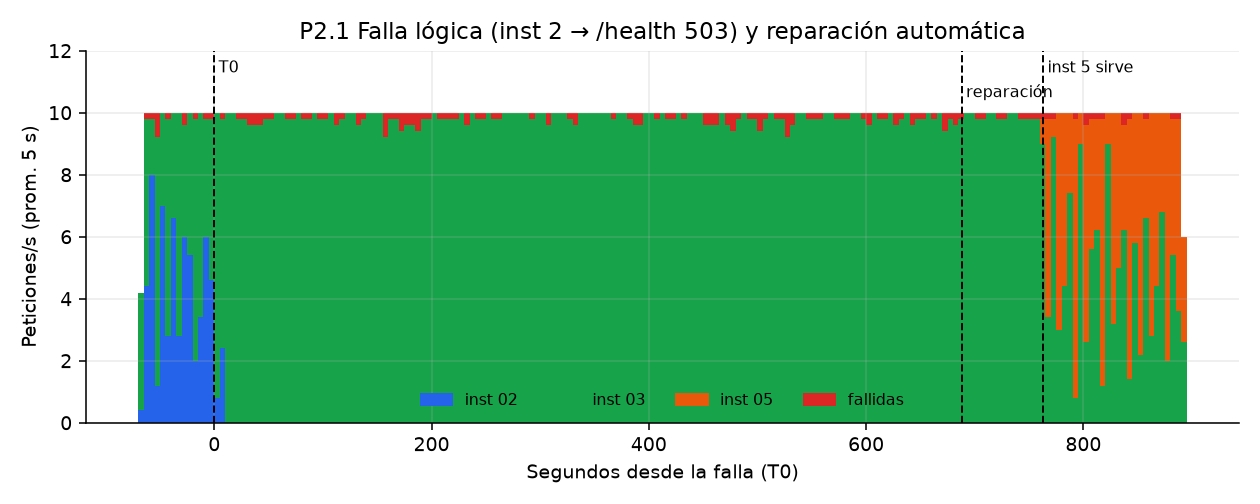
\includegraphics[width=\linewidth]{figuras/p2_logica.png}
\caption{Falla lógica.}
\end{subfigure}\hfill
\begin{subfigure}{0.49\textwidth}
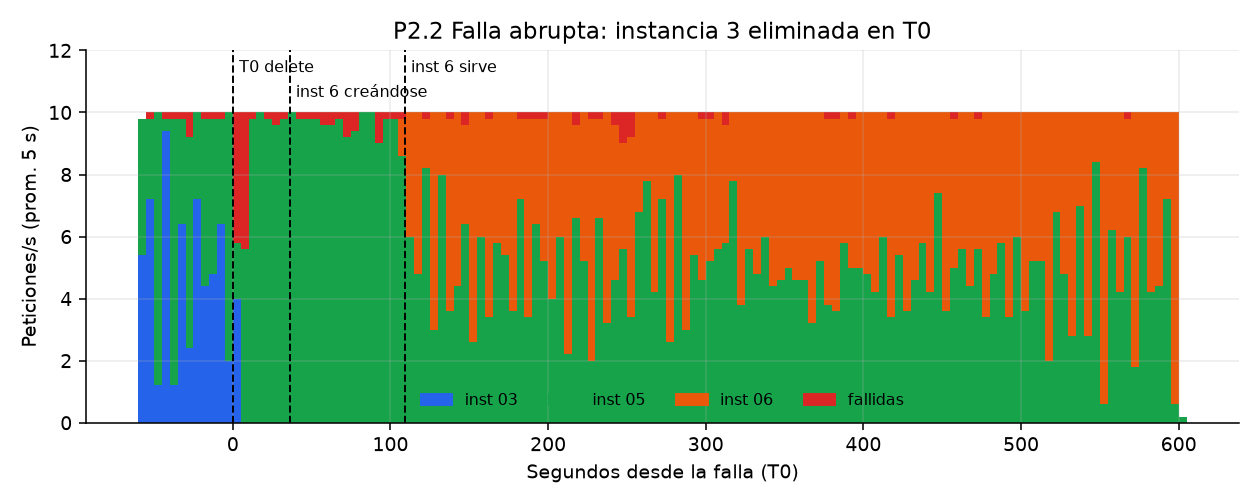
\includegraphics[width=\linewidth]{figuras/p2_abrupta.png}
\caption{Falla abrupta.}
\end{subfigure}
\caption{Peticiones por segundo que atendió cada servidor (colores) y las fallidas (rojo).}
\label{fig:p2}
\end{figure}

\begin{figure}[H]
\centering
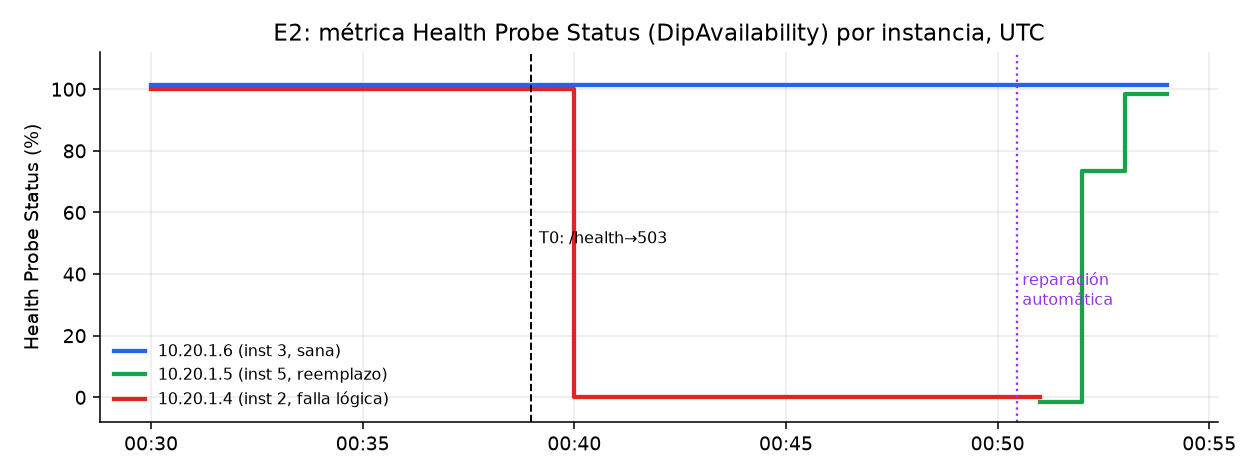
\includegraphics[width=0.6\textwidth]{figuras/e2_health_probe.png}
\caption{Salud de cada servidor según el balanceador: el servidor con falla queda en 0\,\% hasta que lo reemplazan.}
\label{fig:p2logica}
\end{figure}

\textbf{Análisis.} La falla lógica pasó desapercibida para los usuarios: el servidor siguió
respondiendo lo que tenía en curso mientras el balanceador lo retiraba, y el porcentaje de error
no cambió (esos pocos errores vienen de nuestra red doméstica y ya estaban antes de la falla). La
falla abrupta sí se notó, pero solo unos 15 segundos: es lo que tarda el balanceador en confirmar,
con dos revisiones de 5\,s, que el servidor ya no existe. Con más servidores en línea, la parte
afectada del tráfico sería menor. La reparación automática fue lenta (11 minutos) porque Azure
espera 10 minutos antes de reemplazar; el autoscale, en cambio, repuso la capacidad en menos de
2 minutos.


\subsection{P3 ¿Resisten los controles de seguridad?}
\begin{enumerate}
  \item \textbf{Leer el secreto desde otra red.} Desde Azure Cloud Shell, con un usuario que
        \emph{sí} tiene permiso sobre el Key Vault, la lectura fue rechazada por el firewall
        (\texttt{ForbiddenByFirewall}). Tener el permiso no basta: también hay que estar en una
        red autorizada.
  \item \textbf{Salir a Internet desde un servidor.} Desde dentro de una instancia, los intentos de
        conectar con \texttt{example.com} o \texttt{github.com} quedaron sin respuesta, mientras
        que el Key Vault sí respondió. El puerto SSH existe dentro de la máquina, pero no se puede
        alcanzar desde fuera.
  \item \textbf{Romper la política.} Intentamos crear una tarjeta de red con IP pública y un recurso
        en otra región; Azure rechazó ambos (Listado~\ref{lst:policy}).
\end{enumerate}

\begin{lstlisting}[caption={P3.3: Azure Policy rechaza los recursos prohibidos (salida abreviada).},label={lst:policy},language={}]
$ az network nic create ... --public-ip-address pip-prueba-violacion
ERROR: (RequestDisallowedByPolicy) ... "CaribeShop - Denegar NICs con IP publica"
$ az network nsg create ... -l westus
ERROR: (RequestDisallowedByPolicy) ... "CaribeShop - Solo region eastus"
\end{lstlisting}

\subsection{DevSecOps: un cambio inseguro bloqueado}
Cada cambio al código pasa por GitHub Actions, que revisa formato, validez y seguridad (Checkov).
Para comprobarlo abrimos a propósito un pull request que dejaba SSH abierto a Internet: Checkov lo
detectó (\texttt{CKV\_AZURE\_10}), el pipeline falló y el cambio no entró. Un segundo pull request
lo corrigió, usando el acceso de soporte de Azure en lugar de SSH, y se aprobó en verde.

\subsection{Auditoría (S6) y alertas (E5)}
\begin{lstlisting}[caption={S6: consulta KQL de lecturas del secreto y resultado.},label={lst:kql},language={}]
AzureDiagnostics
| where ResourceProvider == 'MICROSOFT.KEYVAULT' and OperationName == 'SecretGet'
| summarize Lecturas=count() by Identidad, Tipo=identity_claim_idtyp_s, Resultado=ResultSignature
-----------------------------------------------------------------------------------
Identidad             Tipo   Lecturas   Resultado
MI vmss-caribeshop    app    5          OK
operador (usuario)    user   1          OK
\end{lstlisting}

La consulta confirma que quien lee el secreto es la identidad de los servidores, desde la red
autorizada. Las alertas se dispararon cuando correspondía y llegaron por correo (Tabla~\ref{tab:alertas}).

\begin{table}[H]
\centering\small\tablaestilo
\caption{Alertas disparadas durante las pruebas.}
\label{tab:alertas}
\begin{tabular}{|l|c|c|c|}
\hline
\encab \hd{Alerta} & \hd{Gravedad} & \hd{Se activó (UTC)} & \hd{Se resolvió (UTC)} \\ \hline
Sonda de salud por debajo de 100\,\% & 2 & 23:14 & 23:30 \\ \hline
CPU alta sostenida & 3 & 23:53 & 00:00 \\ \hline
Sonda de salud por debajo de 100\,\% & 2 & 23:57 & 00:05 \\ \hline
Sonda de salud por debajo de 100\,\% & 2 & 00:12 & 00:26 \\ \hline
Sonda de salud por debajo de 100\,\% (P2.1) & 2 & 00:42 & 01:06 \\ \hline
\end{tabular}
\end{table}
